\chapter{Experiments}

\section{Tools used}

\subsection{Hardware}
Deep learning models were trained on a machine with Intel i7-6800K hexacore CPU with an NVIDIA GPU GTX 1080 GPU. Development was done on my personal laptop, a 2014 MacBook Pro with Intel i5 Core.

\subsection{Deep Learning Framework}
There are many libraries available for implementing neural networks. The most common among them are TensorFlow\cite{noauthor_TensorFlow:_2018}, Keras\cite{noauthor_keras_nodate}, PyTorch\cite{noauthor_pytorch_nodate}, CNTK\cite{noauthor_microsoft_2018}, MXNet\cite{noauthor_incubator-mxnet:_2018}. Due to its heavy popularity in tutorials, I drilled down to choosing between Keras and TensorFlow. Keras is a high-level abstraction, and can be used in combination with either of TensorFlow or Pytorch. Keras is easy to learn for a beginner, and well documented, with many standard networks to be easily implemented with a few lines of code. However, I chose to use TensorFlow, with the notion that I might have to build networks that are much complicated. For more complicated implementations, Keras does not have straightforward solutions, and TensorFlow is recommended. 
Finally, TensorFlow version 1.9 for GPU was used in this work.

Additional requirements for the smooth working of TensorFlow for GPU are CUDA and CuDNN. CUDA version 9.0 and CuDNN version 7.0 were installed on the systems.

\subsection{Language and environment}
R and Python were considered for development. Python 3.5 was used for the project as Python is more efficient when handling large datasets, and better compared to R from a deployment perspective.
Initially, I used Jupyter Notebooks for exploration and development. However, Jupyter prvoed to be inefficient while deploying code, and I shofted to using Python files in a basic code editor, Sublime Text\cite{noauthor_sublime_nodate}. 

\subsection{Version control and Tracking}
In order to keep track of progress and the several version, I used git. In order to facilitate transition between the 2 machines I worked on, I decided to use Github. All the development code is present in \url{https://github.com/pattern-recogniser/pedestrian-trajectory-predictor}


It is evident that there is heavy research being done for trajectory prediction in the domain of crowd forecasting, and subsequently the majority of data sources come from crowd surveillance. 
Several trajectory datasets were considered. However, as it would be best to use a source that would give the most data, I decided to use the dataset from Socially Aware Crowd Forecasting. 
An interesting point to be noted is that in the case of pedestrian trajectory prediction in a traffic setting, there are no benchmark datasets.
\begin{table}[]
\begin{tabular}{|l|l|l|}
\hline
Dataset     & Domain            & \# of pedestrians \\
\hline
ETH**       & Crowd forecasting      & 360          \\
\hline
UCY*        & Crowd forecasting      & 204          \\
\hline
Zara-01*    & Crowd forecasting      & 204          \\
\hline
Zara-02*    & Crowd forecasting      & 207          \\
\hline
Social-LSTM & Crowd forecasting      & 14k          \\
\hline
Poly-MLP    & Pedestrian \& Cyclists & 1068 pedestrian, 464 cyclist trajectories\\
\hline
\end{tabular}
\caption{Datasets considered}
\label{table:dataset_considered}

\end{table}
\section{Experimental Setup}
\section{Dataset}

The dataset used is a set of trajectories collected from a train station from the work of Alahi et al. \cite{alahi_socially-aware_2014}. It consists of 42 million trajectories. 
The data is split across 13 files that are in .csv format, with each file having around <insert number here> number of rows. Each file represents one day's recorded data. The data is sampled at 100 millisecond intervals. Each row in the .csv file is a combination of time-stamp, x-co-ordinate and y-coordinate position in millimetres from the origin, which is the top left of the image. There are on average <insert number here> of pedestrians in each file
\begin{figure}
    \centering
    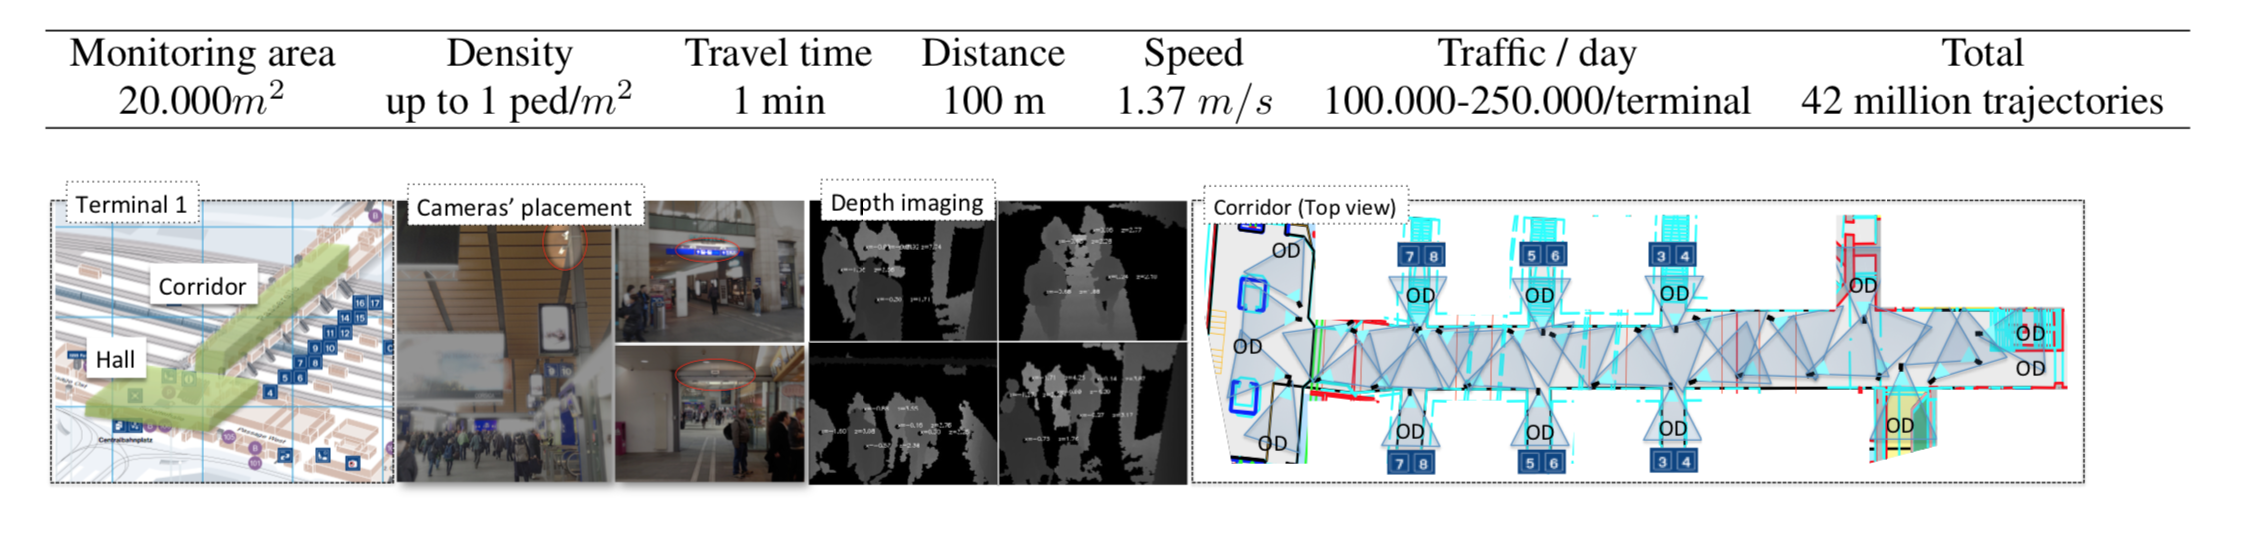
\includegraphics[width=\textwidth]{Figures/Dataset_explanation.png}
    \caption[Key info of Dataset used]{Real-world setup. Top row presents some facts regarding the dataset (values are in average). Bottom row illustrates one of the monitored corridors. More than 30 cameras are deployed in the presented corridor, whereas 132 cameras are deployed in total in 3 corridors, one track, and one large hall. At any given time, the occupancy of the corridor can reach more than one thousand of pedestrians. The label 'OD' represents entry/exit zones }

    \label{fig:dataset_explanation}
\end{figure}

\section{Data Handling}
Data is processed and stored on file as a processed pickle.
Data is read in by keeping only 




\section{Data Cleaning}
\begin{itemize}
    \item Assigning a trajectory ID:
    
    The same pedestrian if observed after a span of 2 minutes is considered as a different trajectory.
    
    \item Removing Outliers:
    
    If consecutive x co-ordinate or y-co-ordinate positions differ by more than 500 millimetres, we consider these as another trajectory. This is equivalent to capping the speed of a walking person to \(5 m/s\)
    
    \item Normalisation
    

\end{itemize}

Data is split into train:test:dev set using a 98:1:1 split.
Final reported metrics are from the test set. Results of loss from the dev set are also reported in this document. However, as a performance metric, only the test set metric is used.









